\chapter{Практическая часть}
\section{Код программы}
Модуль разработанных алгоритмов представлен на листинге \ref{lst:code}
\begin{lstlisting}[label=lst:code, caption=Модуль разработанных алгоритмов, basicstyle=\footnotesize]
##Тартыков Лев ИУ7-64Б, 2022 г
pkg load statistics;
echo off all;

function main()
	[error, X] = load_data("data.txt");
	if (error == 0)
		[bins, counts, count_X, delta, Xn, Y_normpdf, Y_normcdf, Y_ecdf, M_min, M_max, X_without_double, J, count_elem_J] = perform_params(X);
		plot_graphs(bins, counts, count_X, delta, Xn, Y_normpdf, Y_normcdf, Y_ecdf, M_min, M_max, X_without_double, J, count_elem_J);
	endif   
endfunction

function [error, X] = load_data(file_name)
	X = []; i = 1; error = 0;
	file = fopen(file_name, "r");
	if (file == -1)
		error = -1;
	else
		end_file = 0;
		while (end_file == 0)
			if (feof(file))
				end_file = 1;
			else
				X(i) = fscanf(file, '%f', [1,1]);
				fscanf(file, '%c', [1, 1]);
				i++;
			endif
		endwhile
	endif
	fclose(file);
endfunction

function [bins, counts, count_X, delta, Xn, Y_normpdf, Y_normcdf, Y_ecdf, M_min, M_max, X_without_double, J, count_elem_J] = perform_params(X)
	count_X = length(X);
	M_max = max(X)
	M_min = min(X)
	
	R = M_max - M_min;
	MX = find_MX(X, count_X);
	DX = find_DX(X, MX, count_X);
	
	m = find_m(count_X);
	output_results(M_max, M_min, R, MX, DX, m);
	[counts, bins] = hist(X, m);
	
	delta = R / m;
	sigma = sqrt(DX);
	abs_MX = abs(MX);
	[J, count_elem_J] = calc_hist(X, M_min, M_max, delta);
	M_min = M_min - abs_MX / 2;
	M_max = M_max + abs_MX / 2;
	Xn = M_min:delta/20:M_max;
	
	Y_normpdf = density_ndist(Xn, MX, sigma);
	Y_normcdf = form_normcdf(Xn, MX, sigma);
	[count_elem, X_without_double] = count_number_elems(X, count_X, M_min, M_max);
	Y_ecdf = form_y_ecdf(count_elem, count_X, M_min, M_max);
endfunction

function [MX] = find_MX(X, count_X)
	MX = sum(X) / count_X;
endfunction

function [DX] = find_DX(X, MX, count_X)
	DX = sum((X - MX).^2) / (count_X - 1);
endfunction

function [m] = find_m(count_X)
	m = floor(log2(count_X)) + 2;
endfunction

function [J, count_elem_J] = calc_hist(X, M_min, M_max, delta)
	J = (M_min - delta): delta: (M_max + delta);
	count_elem_J = [];
	len_J = length(J);
	len_X = length(X);
	for i = 2: len_J - 2
		count_elem = 0;
		for j = 1: len_X
			if ((X(j) > J(i)) || abs(X(j) - J(i)) <= 1e-3)
				if ((i == len_J - 2) && (X(j) < J(i + 1) ||  
					(abs(X(j) - J(i + 1))) <= 1e-3))
					count_elem += 1;
				elseif (X(j) < J(i + 1))
					count_elem += 1;
				endif
			endif
		endfor
		count_elem_J(i) = count_elem;
	endfor
	count_elem_J(len_J) = 0;
endfunction

function [Y_normpdf] = density_ndist(Xn, MX, sigma)
	Y_normpdf = [];
	count_X = length(Xn);
	for i = 1: count_X
		Y_normpdf(i) = \
			1 / (sqrt(2 * pi) * sigma) * exp(-(Xn(i) - MX).^2 / (2 * sigma.^2));
	endfor
endfunction

function [count_elem, X_graph] = count_number_elems(X, count_X, M_min, M_max)
	X_sort = sort(X);
	count_elem = [];
	X_without_double = [];
	i = 1;
	index_count = 1;
	while (i < count_X)
		is_all = 0;
		temp_value = X_sort(i);
		j = 1;
		while (is_all == 0)
			if (X_sort(i + j) == temp_value && i + j < count_X)
				j++;
			else
				is_all = 1;
			endif
		endwhile
		X_without_double(index_count) = temp_value;
		count_elem(index_count) = j;
		index_count += 1;
		i += j; 
	endwhile

	if (X_sort(count_X) != X_sort(count_X - 1))
		count_elem(index_count) = 1;
		X_without_double(index_count) = X_sort(count_X);
	endif

	X_graph = [];
	X_graph(1) = X_without_double(1) - abs(M_min);
	X_graph(2) = X_without_double(1);
	X_graph(3) = X_graph(2);
	j = 4;
	for i = 2: length(X_without_double)
		X_graph(j) = X_without_double(i);
		X_graph(j + 1) = X_without_double(i);
		j += 2;
	endfor
	X_graph(j) = abs(M_max);  
endfunction

function [Y_normcdf] = form_normcdf(Xn, MX, sigma)
	Y_normpdf = \
	 @(Xn) ((1./(sqrt(2.*pi).*sigma)).*(exp((-0.5.*(Xn - MX).^2)./(sigma.^2))));
	 
	for k = 1: length(Xn)
		Y_normcdf(k) = integral(Y_normpdf, -inf, Xn(k));
	endfor
endfunction

function [Y_ecdf] = form_y_ecdf(count_elem, count_X)
	Y_ecdf = [];
	len_celem = length(count_elem);

	Y_ecdf(1) = 0;
	Y_ecdf(2) = 0;
	Y_ecdf(3) = count_elem(1) / count_X;
	Y_ecdf(4) = Y_ecdf(3);
	j = 5;
	for i = 2: len_celem
		Y_ecdf(j) = Y_ecdf(j - 1) + count_elem(i) / count_X;
		Y_ecdf(j + 1) = Y_ecdf(j);
		j += 2;
	endfor
endfunction

function plot_graphs(bins, counts, count_X, delta, Xn, Y_normpdf, Y_normcdf, Y_ecdf, M_min, M_max, X_without_double)
	figure;
	subplot(1, 2, 1);
	stairs(J, count_elem_J / (count_X * delta));
	hold on;
	plot(Xn, Y_normpdf, 'LineWidth', 3, 'Color', 'green');
	xlim([M_min, M_max]);
	hold on;
	
	subplot(1, 2, 2);
	plot(Xn, Y_normcdf, 'LineWidth', 1, 'Color', 'red');
	xlim([M_min, M_max]);
	hold on;
	plot(X_without_double, Y_ecdf, 'LineWidth', 1, 'Color', 'blue');
	xlim([M_min, M_max]);
endfunction

function output_results(M_min, M_max, R, MX, DX, m)
	fprintf("M_min = %f,\nM_max = %f,\nR = %f,\nMX = %f,\nDX = %f,\nm = %f\n",
			 M_min, M_max, R, MX, DX, m);
endfunction

main()
\end{lstlisting}

\newpage
\section{Результаты расчетов для выборки из индивидуального варианта.}
Согласно варианту 15, результаты расчетов для выборки приведены на формулах (\ref{eq:res_min}), (\ref{eq:res_max}), (\ref{eq:res_r}), (\ref{eq:res_mx}), (\ref{eq:res_dx}), (\ref{eq:res_m}).
\begin{equation}
	\label{eq:res_min}
	M_{\min} = -6.48
\end{equation}
\begin{equation}
	\label{eq:res_max}
	M_{\max} = -1.51
\end{equation}
\begin{equation}
	\label{eq:res_r}
	R = 4.97
\end{equation}
\begin{equation}
	\label{eq:res_mx}
	\hat\mu(\vec x_n) = -3.676
\end{equation}
\begin{equation}
	\label{eq:res_dx}
	S^2(\vec x_n) = 0.866
\end{equation}
\begin{equation}
	\label{eq:res_m}
	m = 8
\end{equation}

На рисунке \ref{image:graph1} представлены гистограмма и график функции плотности распределения вероятностей нормальной случайной величины с выборочными мат. ожиданием и дисперсией.
\begin{figure}[H]
	\centering{
		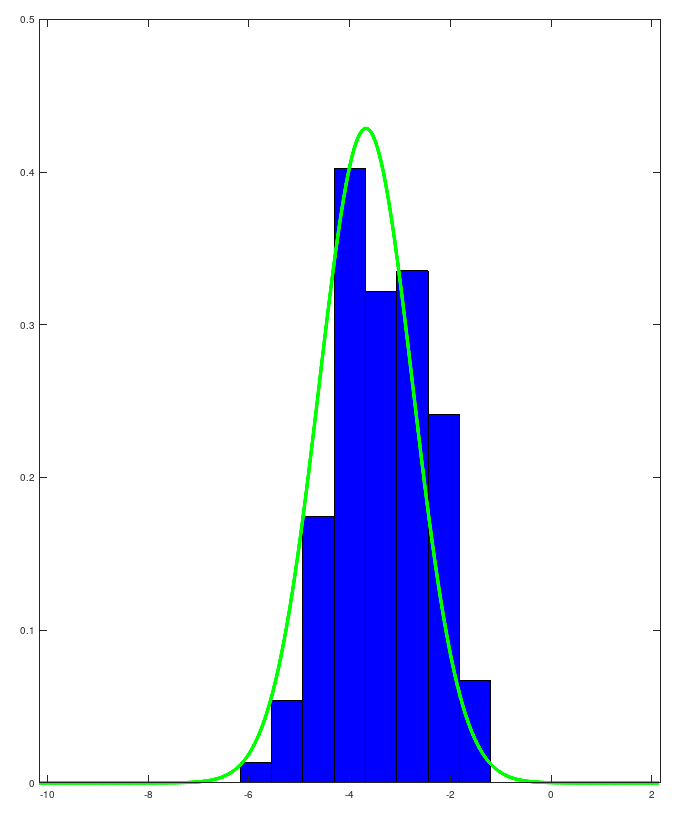
\includegraphics[scale=0.5]{./images/graph_1}
		\caption{Гистограмма и график функции плотности распределения вероятностей нормальной случайной величины с выборочными мат. ожиданием и дисперсией.}
		\label{image:graph1}
	}
\end{figure}

На рисунке \ref{image:graph2} представлены график эмпирической функции распределения и функции распределения нормальной случайной величины с выборочными мат. ожиданием и дисперсией.
\begin{figure}[H]
	\centering{
		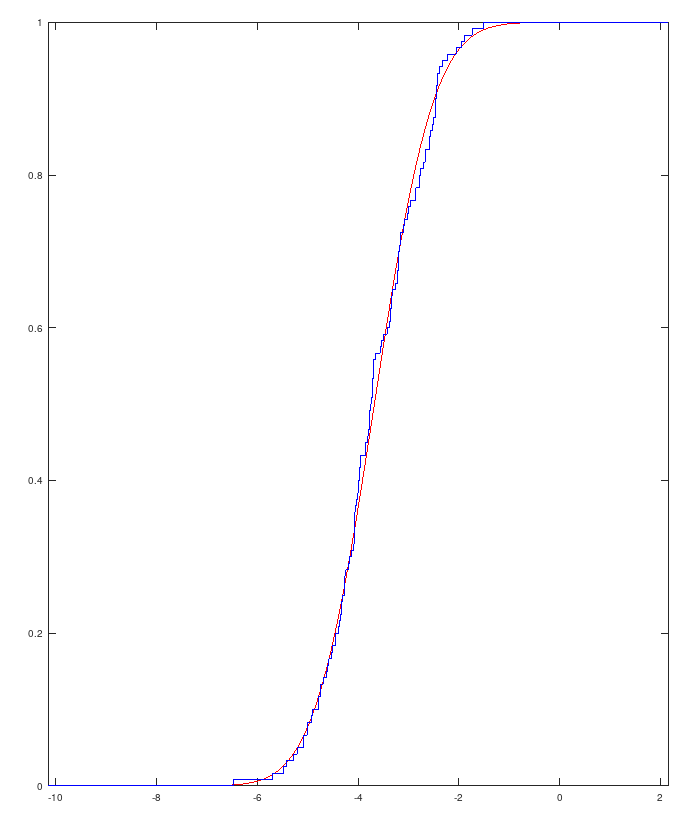
\includegraphics[scale=0.5]{./images/graph_2}
		\caption{График эмпирической функции распределения и функции распределения нормальной случайной величины с выборочными мат. ожиданием и дисперсией.}
		\label{image:graph2}
	}
\end{figure}